
\section{Introduction}\label{sec-intro}


The analysis of time trends is an important aspect of many time series applications. In a wide range of situations, practitioners are particularly interested in certain shape properties of the trend. They raise questions such as the following: Does the observed time series have a trend at all? If so, is the trend increasing/decreasing in certain time \textcolor{red}{intervals}? Can one identify the \textcolor{red}{intervals} of increase/decrease? As an example, consider the time series plotted in Figure \ref{temp_data} which shows the yearly mean temperature in Central England from 1659 to 2017. Climatologists are very much interested in learning about the trending behaviour of temperature time series like this; see e.g.\ \cite{Benner1999} and \cite{Rahmstorf2017}. Among other things, they would like to know whether there is an upward trend in the Central England mean temperature towards the end of the sample as visual inspection might suggest.


\begin{figure}
\centering
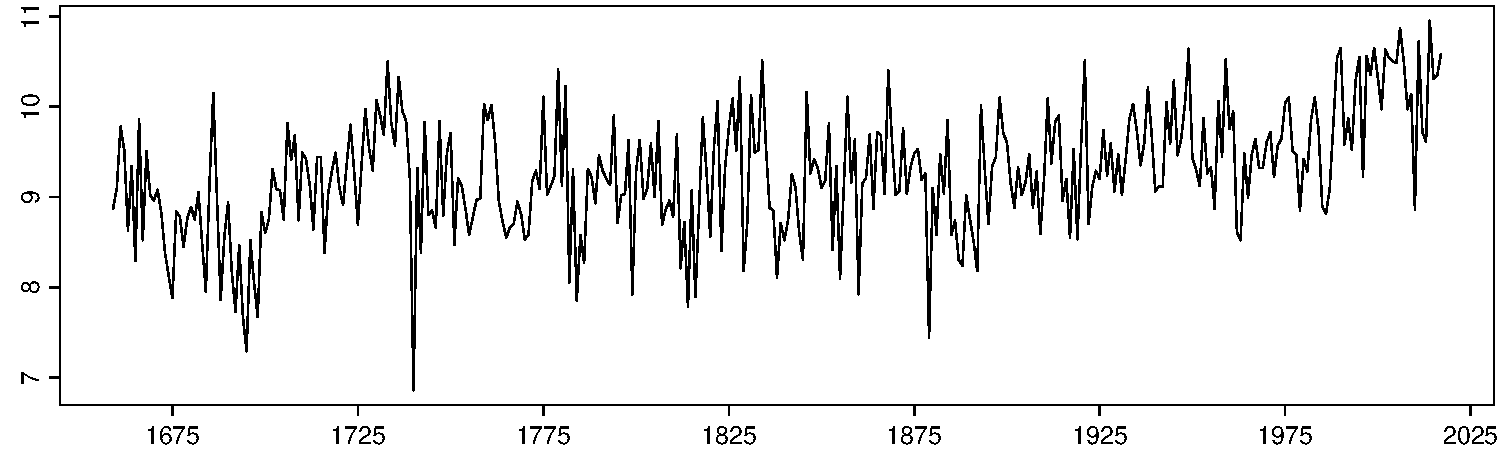
\includegraphics[width=0.9\textwidth]{Plots/temp_data.pdf}
\vspace{0.15cm}

\caption{Yearly mean temperature in Central England from 1659 to 2017 measured in $^\circ$C.}\label{temp_data}
\end{figure}


In this paper, we develop new methods to test for certain shape properties of a nonparametric time trend. We in particular construct a multiscale test which allows to identify local increases/decreases of the trend function. 
%We in particular construct a multiscale test for local increases/de\-creases of the trend function. The proposed test allows to identify, with a pre-specified statistical confidence, time regions where there is an increase/decrease in the trend. 
%identify subintervals on which the function $m$ deviates significantly from the null hypothesis of constancy. 
We develop our test in the context of the following model setting: We observe a time series $\{ Y_{t,T}: 1 \le t \le T \}$ of the form 
\begin{equation}\label{model-intro}
Y_{t,T} = m \Big( \frac{t}{T} \Big) + \varepsilon_t
\end{equation}
for $1 \le t \le T$, where $m: [0,1] \rightarrow \mathbb{R}$ is an unknown nonparametric regression function and the error terms $\varepsilon_t$ form a stationary time series process with $\ex[\varepsilon_t] = 0$. In a time series context, the design points $t/T$ represent the time points of observation and $m$ is a nonparametric time trend. As usual in nonparametric regression, we let the function $m$ depend on rescaled time $t/T$ rather than on real time $t$. A detailed description of model \eqref{model-intro} is provided in Section \ref{sec-model}.


Our multiscale test is developed step by step in Section \ref{sec-method}. Roughly speaking, the procedure can be outlined as follows: Let $H_0(u,h)$ be the hypothesis that $m$ is constant in the time window $[u-h,u+h] \subseteq [0,1]$, where $u$ is the midpoint and $2h$ the size of the window. In a first step, we set up a \textcolor{red}{test statistic $\widehat{\varphi}_T(u,h)$} for the hypothesis $H_0(u,h)$. In a second step, we aggregate \textcolor{red}{the statistics $\widehat{\varphi}_T(u,h)$} for a large number of different time windows $[u-h,u+h]$. We thereby construct a multiscale statistic which allows to test the hypothesis $H_0(u,h)$ simultaneously for many time windows $[u-h,u+h]$. In the technical part of the paper, we derive the theoretical properties of the resulting multiscale test. To do so, we come up with a proof strategy which combines strong approximation results for dependent processes with anti-concentration bounds for Gaussian random vectors. This strategy is of interest in itself and may be applied to other multiscale test problems for dependent data. As shown by our theoretical analysis, our multiscale test is a rigorous level-$\alpha$-test of the overall null hypothesis $H_0$ that $H_0(u,h)$ is simultaneously fulfilled for all time windows $[u-h,u+h]$ under consideration. Moreover, for a given significance level $\alpha \in (0,1)$, the test allows to make simultaneous confidence statements of the following form: We can claim, with statistical confidence $1-\alpha$, that there is an increase/decrease in the trend $m$ on all time windows $[u-h,u+h]$ for which the hypothesis $H_0(u,h)$ is rejected. Hence, the test allows to identify, with a pre-specified statistical confidence, time \textcolor{red}{intervals} where the trend $m$ is increasing/decreasing. 


For independent data, multiscale tests have been developed in a variety of different contexts in recent years. In the regression context, \cite{ChaudhuriMarron1999,ChaudhuriMarron2000} introduced the so-called SiZer method which has been extended in various directions; see e.g.\ \cite{HannigMarron2006} where a refined distribution theory for SiZer is derived. \cite{HallHeckman2000} constructed a multiscale test on monotonicity of a regression function. \cite{DuembgenSpokoiny2001} developed a multiscale approach which works with additively corrected supremum statistics and derived theoretical results in the context of a continuous Gaussian white noise model. Rank-based multiscale tests for nonparametric regression were proposed in \cite{Duembgen2002} and \cite{Rohde2008}. More recently, \cite{ProkschWernerMunk2018} have constructed multiscale tests for inverse regression models. In the context of density estimation, multiscale tests have been investigated in \cite{DuembgenWalther2008}, \cite{RufibachWalther2010}, \cite{SchmidtHieber2013} and \cite{EckleBissantzDette2017} among others. 


Whereas a large number of multiscale tests for independent data have been developed in recent years, multiscale tests for dependent data are much rarer. Most notably, there are some extensions of the SiZer approach to a time series context. \cite{Rondonotti2004} and \cite{Rondonotti2007} have introduced SiZer methods for dependent data which can be used to find local increases/decreases of a trend and which may thus be regarded as an alternative to our multiscale test. However, these SiZer methods are mainly designed for data exploration rather than for rigorous statistical inference. Our multiscale method, in contrast, is a rigorous level-$\alpha$-test of the hypo\-thesis $H_0$ which allows to make simultaneous confidence statements about the time \textcolor{red}{intervals} where the trend $m$ is increasing/decreasing. Some theoretical results for dependent SiZer methods have been derived in \cite{ParkHannigKang2009}, but only under a quite severe restriction: Only time windows $[u-h,u+h]$ with window sizes or scales $h$ are taken into account that remain bounded away from zero as the sample size $T$ grows. Scales $h$ that converge to zero as $T$ increases are excluded. This effectively means that only large time windows $[u-h,u+h]$ are taken into consideration. Our theory, in contrast, allows to simultaneously consider scales $h$ of fixed size and scales $h$ that converge to zero at various different rates. We are thus able to take into account time windows of many different sizes. \textcolor{red}{In Section \ref{subsec-method-comparison}, we compare our approach to SiZer methods for dependent data in more detail.}


Our multiscale approach is also related to Wavelet-based methods: Similar to the latter, it takes into account different locations $u$ and resolution levels or scales $h$ simultaneously. However, while our multiscale approach is designed to test for local increases/decreases of a nonparametric trend, Wavelet methods are commonly used for other purposes. Among other things, they are employed for estimating/reconstructing nonparametric regression curves [see e.g.\ \cite{Donoho1995} or \cite{vonSachsMacGibbon2000}] and for change point detection [see e.g.\ \citet{ChoFryzlewicz2012}]. 


%Whereas a large number of multiscale tests for independent data have been developed in recent years, multiscale tests for dependent data are much rarer. Most notably, there are some extensions of the SiZer approach to a time series context. \cite{Rondonotti2004}, \cite{Rondonotti2007} and \cite{ParkHannigKang2009} have developed SiZer methods for dependent data which can be regarded as an alternative to our multiscale test. However, these SiZer methods are mainly designed for data exploration rather than rigorous statistical inference. Our multiscale method, in contrast, is a rigorous level-$\alpha$-test of the hypo\-thesis $H_0$, which is backed up by a complete asymptotic theory. Moreover, it allows to make simultaneous confidence statements about the time regions where the trend function $m$ is increasing/decreasing, which is not possible with the SiZer tools of \cite{Rondonotti2004}, \cite{Rondonotti2007} and \cite{ParkHannigKang2009}. Our multiscale approach is also related to Wavelet-based methods: It investigates the data on different intervals $[u-h,u+h]$. Similar to Wavelet-based procedures, it thus takes into account different locations $u$ and resolution levels $h$ simultaneously. Nevertheless, we are not aware of any Wavelet-based test for local increases/decreases of the nonparametric trend function in model \eqref{model-intro}. Wavelet methods have been used for other purposes in the literature such as estimating/reconstructing nonparametric regression functions [see e.g.\ \cite{Donoho1995} or \cite{vonSachsMacGibbon2000}] and change point detection [see e.g.\ \citet{ChoFryzlewicz2012}]. 


The test statistic of our multiscale method depends on the long-run error variance $\sigma^2 = \sum\nolimits_{\ell=-\infty}^{\infty} \cov(\varepsilon_0,\varepsilon_{\ell})$, which is usually unknown in practice. To carry out our multiscale test, we thus require an estimator of $\sigma^2$. Indeed, such an estimator is required for virtually all inferential procedures in the context of model \eqref{model-intro}. Hence, the problem of estimating $\sigma^2$ in model \eqref{model-intro} is of broader interest and has received a lot of attention in the literature; see \cite{MuellerStadtmueller1988}, \cite{Herrmann1992} and \cite{Hall2003} among many others. In Section \ref{sec-error-var}, 
%we discuss several estimators of $\sigma^2$ which are valid under different conditions on the error process $\{\varepsilon_t\}$. 
\textcolor{red}{we introduce a new difference-based estimator of $\sigma^2$ for the case that $\{ \varepsilon_t \}$ belongs to the class of AR($\infty$) processes}. This estimator improves on existing methods in several respects. 


The methodological and theoretical analysis of the paper is complemented by a simulation study in Section \ref{sec-sim} and \textcolor{red}{two empirical applications} in Section \ref{sec-data}. In the simulation study, we examine the finite sample properties of our multiscale test and compare it to the dependent SiZer methods introduced in \cite{Rondonotti2004} and \cite{Rondonotti2007}. \textcolor{red}{Moreover, we investigate the small sample performance of our estimator of $\sigma^2$} and compare it to the estimator of \cite{Hall2003}. In Section \ref{sec-data}, we use our methods to analyse the temperature data from Figure \ref{temp_data} \textcolor{red}{as well as a sample of global temperature data}. 


